\documentclass[a4paper, 11pt]{article}
\usepackage[english]{babel}
\usepackage{fullpage}

\usepackage[pdftex]{graphicx}
\graphicspath{{../pdf/}{../jpeg/}}
\DeclareGraphicsExtensions{.pdf,.jpeg,.png}

% ----------------------------------------------

% Definitions of languages: --------------------
\usepackage{listings}
\lstdefinestyle{cStyle}{
  basicstyle=\scriptsize,
  breakatwhitespace=false,
  breaklines=true,
  captionpos=b,
  keepspaces=true,
  numbersep=5pt,
  showspaces=false,
  gobble=4,
  tabsize=4,
  showstringspaces=false,
  showtabs=false,
}
\renewcommand*{\lstlistingname}{Code}

% ----------------------------------------------

\begin{document}

\noindent
\large\textbf{CES-27 Distributed Processing} \\
\textbf{2nd Activity} \\
\normalsize Prof Hirata and Prof Juliana  \\
Carlos Matheus Barros da Silva \hfill September 2019

\section*{2th Activity}

It was implemented the Ricart-Agrawala's algorithm. The implementation was made in Go, and it can be seen on the repository\footnote{https://github.com/CarlosMatheus/CES-27/tree/master/lab02}.

\section*{First Case}

The first test was conducted with 3 terminal windows on two of them were open the process and on the third one was open the shared process.

The test was made according to the model represented on Figure \ref{img_task1}. The results can be seen on the terminal windows shown from Figure \ref{img_task1_example_window1} to Figure \ref{img_task1_example_window3}.

\begin{figure}[h]
  \begin{center}
  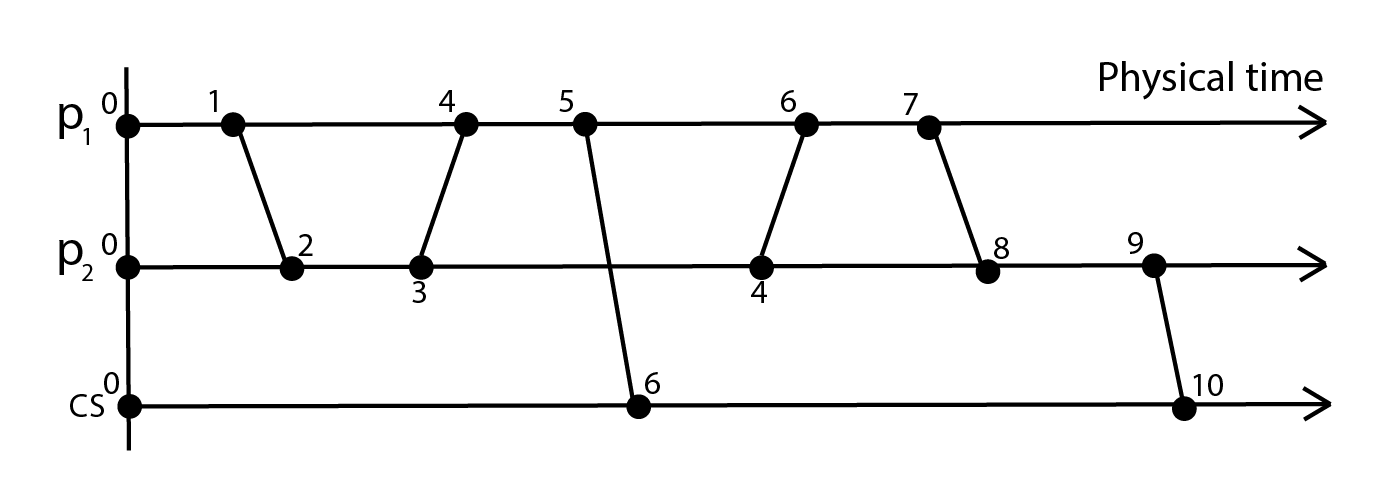
\includegraphics[width=4in]{./imgs/case1.png}
  \caption{Model representing the execution of Case 1.}
  \label{img_task1}
  \end{center}
\end{figure}

\begin{figure}[h]
  \begin{center}
  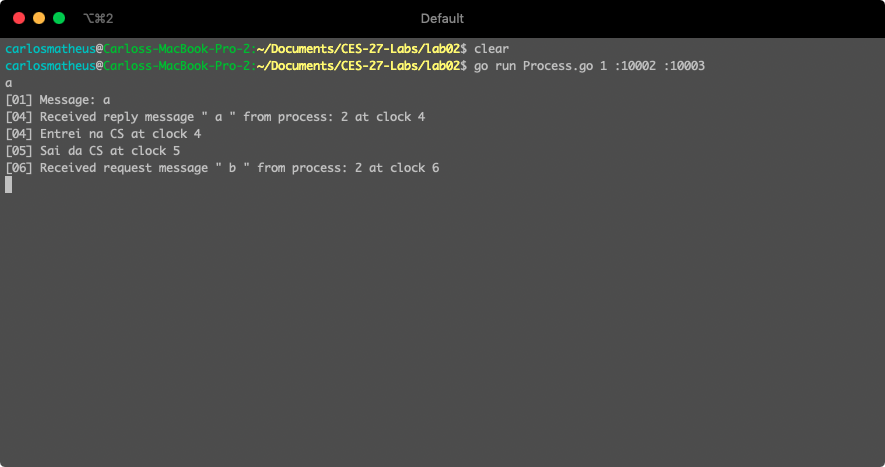
\includegraphics[width=4.5in]{./imgs/case1process1.png}
  \caption{Process 1 after execution of Case 1 example test case.}
  \label{img_task1_example_window1}
  \end{center}
\end{figure}

\begin{figure}[h]
  \begin{center}
  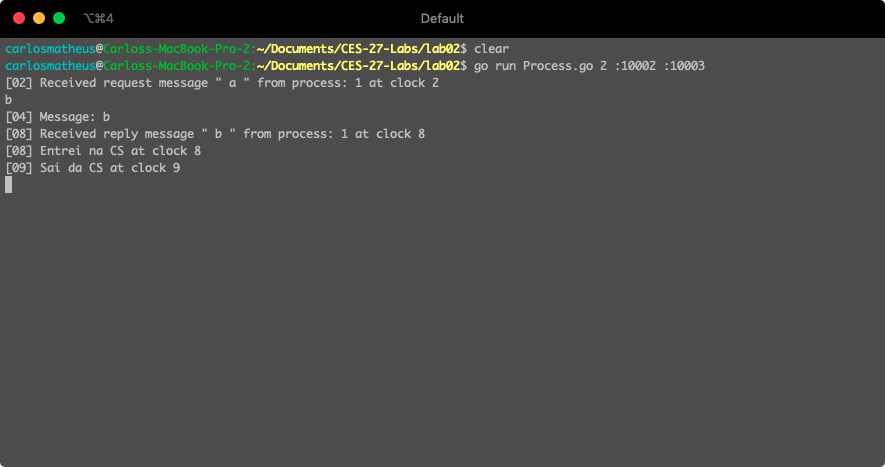
\includegraphics[width=4.5in]{./imgs/case1process2.png}
  \caption{Process 2 after execution of Case 1 example test case.}
  \label{img_task1_example_window2}
  \end{center}
\end{figure}

\begin{figure}[h]
  \begin{center}
  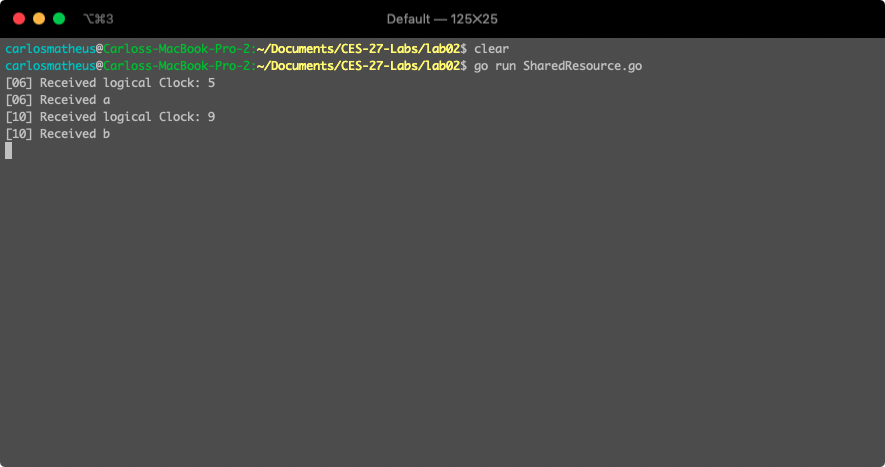
\includegraphics[width=4.5in]{./imgs/case1CS.png}
  \caption{Shared Resource after execution of Case 1 example test case.}
  \label{img_task1_example_window3}
  \end{center}
\end{figure}

As expected, the mutual exclusion worked; thus, when a process request access the other reply allowing the access when it is on \textit{released} state, then the first process accesses the shared resource. When it finishes, it returns to released state. Then the second process does the same steps. All the logic worked as well as the logical clocks on each process; therefore, the simulation on the terminals matched the model represented in Figure \ref{img_task1}.

\section*{Second Case}

It was built a test case with 6 terminal windows. The test was made according to the model represented in Figure \ref{img_task2}. The results can be seen on the terminal windows shown from Figure \ref{img_task2_example_window1} to Figure \ref{img_task2_example_window6}.

\begin{figure}[h]
  \begin{center}
  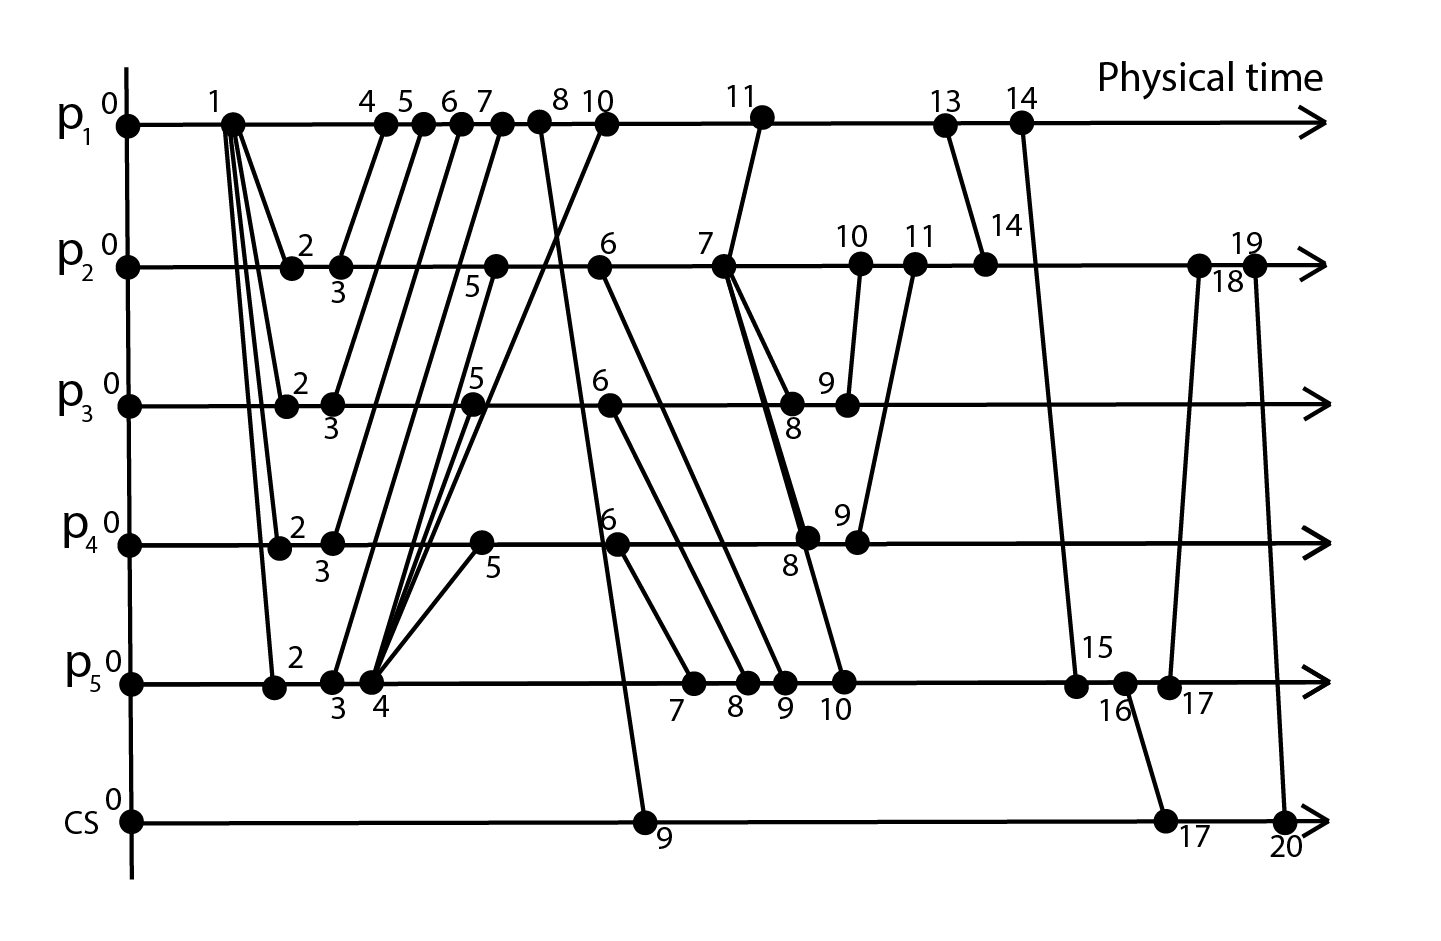
\includegraphics[width=4in]{./imgs/case2.png}
  \caption{Model representing the execution of Case 1.}
  \label{img_task2}
  \end{center}
\end{figure}

\begin{figure}[h]
  \begin{center}
  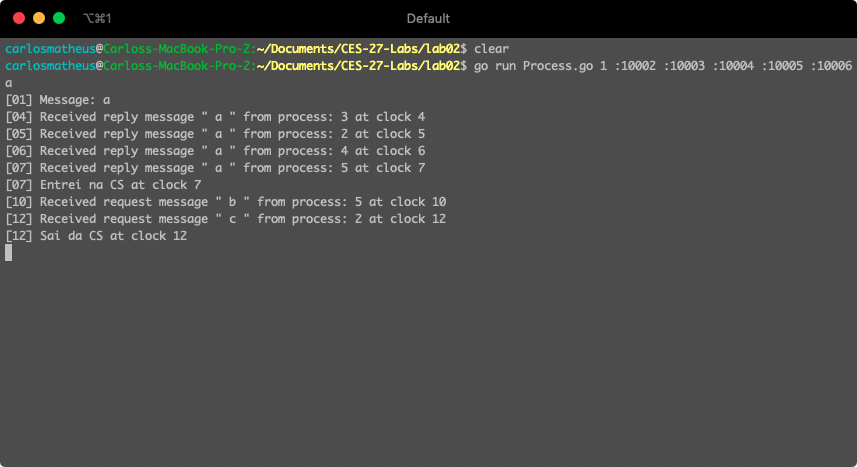
\includegraphics[width=4.5in]{./imgs/case2process1.png}
  \caption{Process 1 after execution of Case 2 example test case.}
  \label{img_task2_example_window1}
  \end{center}
\end{figure}

\begin{figure}[h]
  \begin{center}
  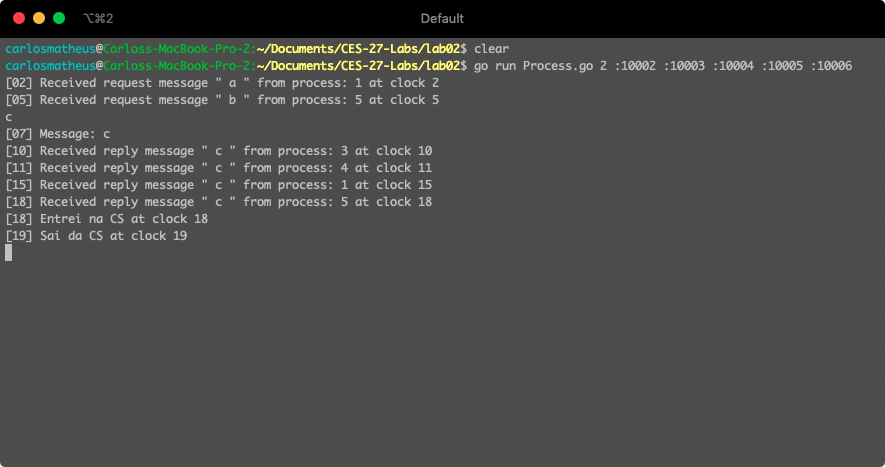
\includegraphics[width=4.5in]{./imgs/case2process2.png}
  \caption{Process 2 after execution of Case 2 example test case.}
  \label{img_task2_example_window2}
  \end{center}
\end{figure}

\begin{figure}[h]
  \begin{center}
  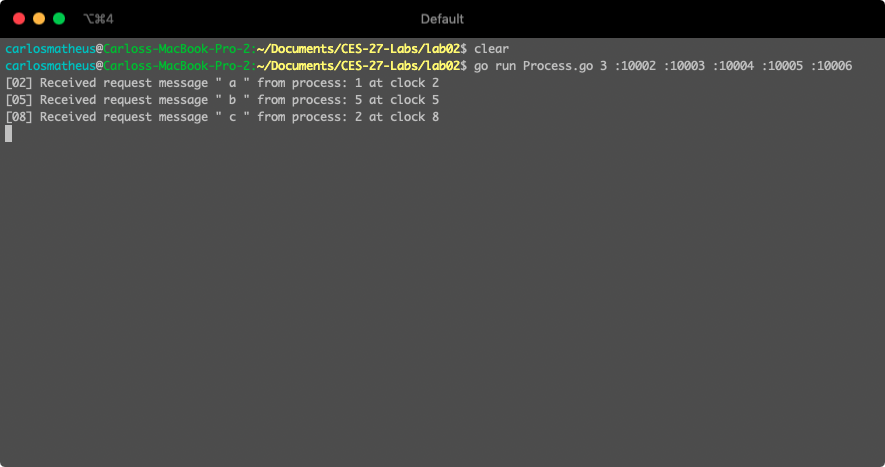
\includegraphics[width=4.5in]{./imgs/case2process3.png}
  \caption{Process 3 after execution of Case 2 example test case.}
  \label{img_task2_example_window3}
  \end{center}
\end{figure}

\begin{figure}[h]
  \begin{center}
  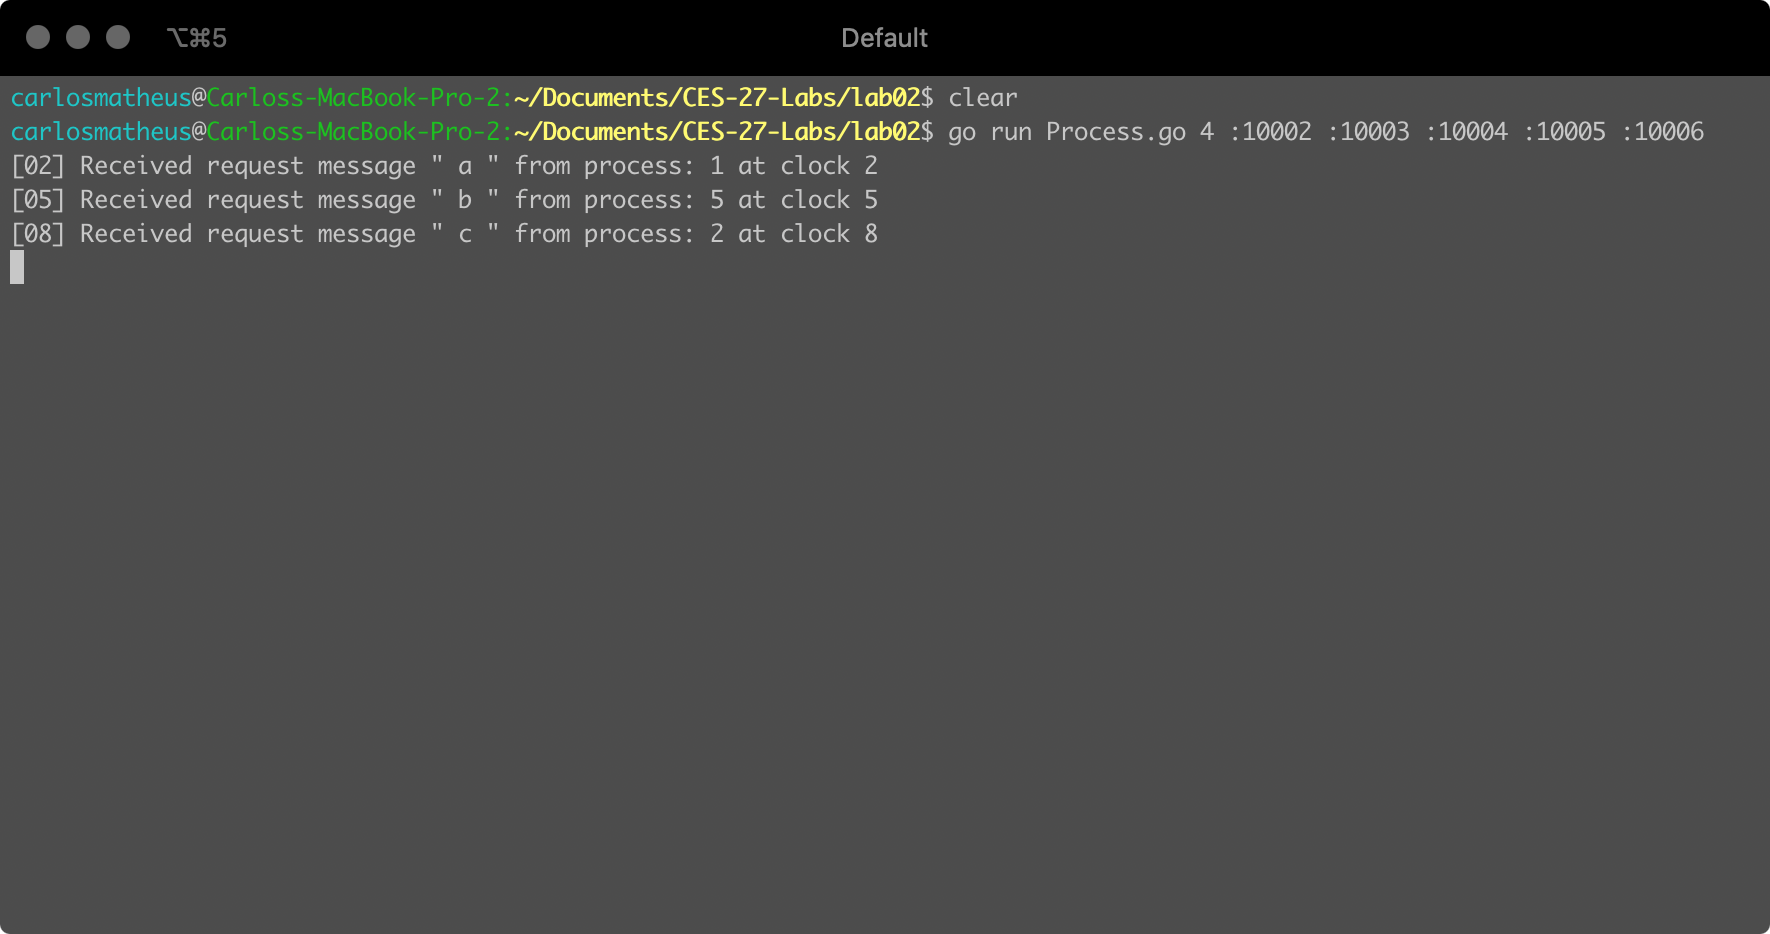
\includegraphics[width=4.5in]{./imgs/case2process4.png}
  \caption{Process 4 after execution of Case 2 example test case.}
  \label{img_task2_example_window4}
  \end{center}
\end{figure}

\begin{figure}[h]
  \begin{center}
  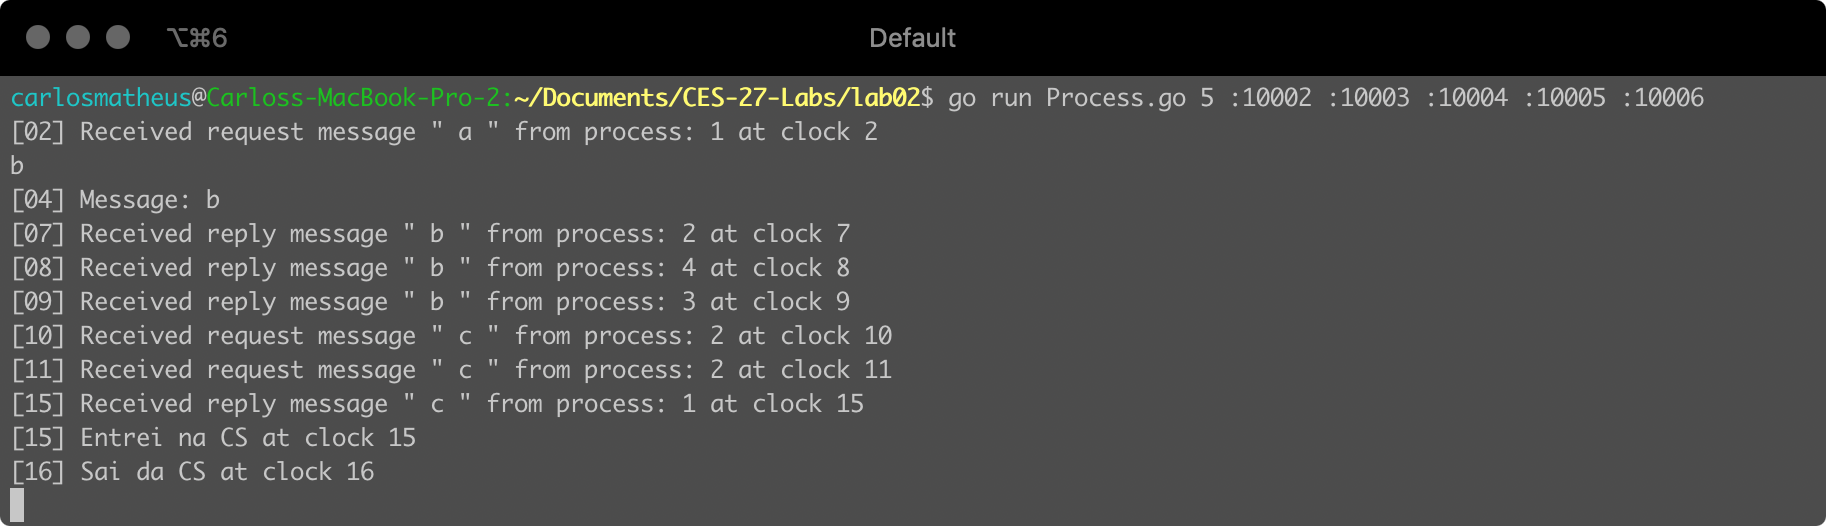
\includegraphics[width=4.5in]{./imgs/case2process5.png}
  \caption{Process 5 after execution of Case 2 example test case.}
  \label{img_task2_example_window5}
  \end{center}
\end{figure}

\begin{figure}[h]
  \begin{center}
  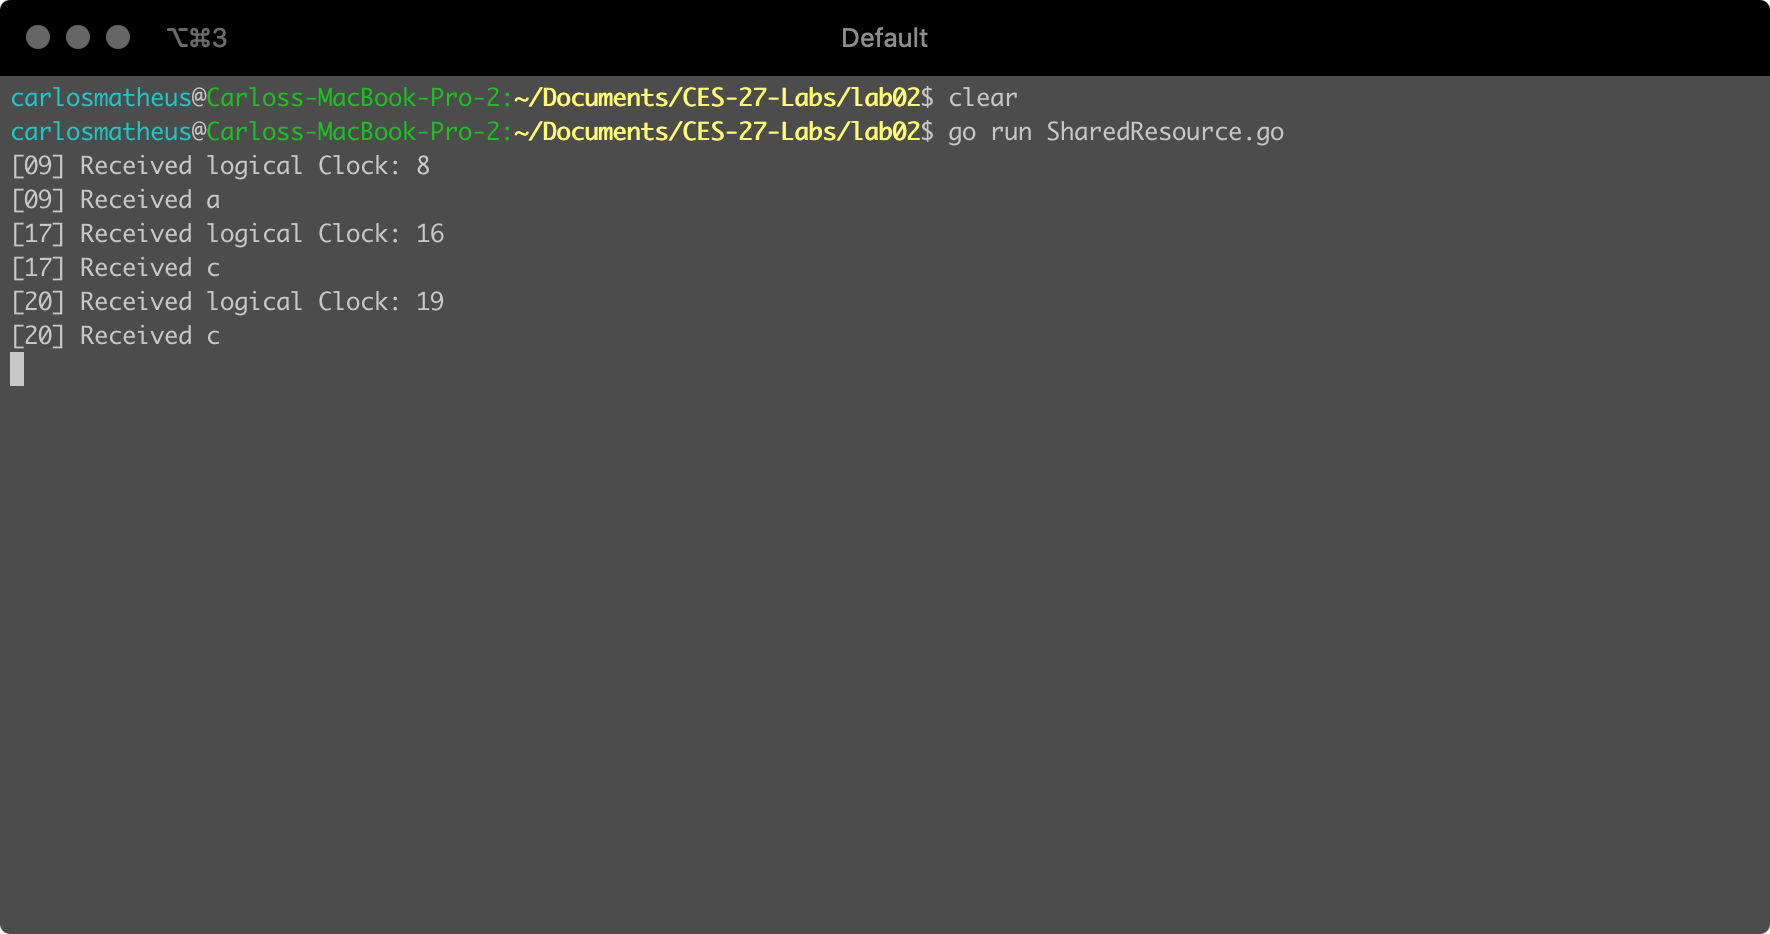
\includegraphics[width=4.5in]{./imgs/case2CS.png}
  \caption{Shared Resource after execution of Case 2 example test case.}
  \label{img_task2_example_window6}
  \end{center}
\end{figure}

As expected, the mutual exclusion worked; Even when multiple processes were wanting to access the shared resource at the same time, the mutual exclusion guaranteed the safety and the liveness of the operation. All the logic worked as well as the logical clocks on each process; therefore, the simulation on the terminals matched the model represented in Figure \ref{img_task2}.


\end{document}
